\section{Biological background}
\label{sec:biol-backgr}

-disease states and bio cond are character by distinct gene expression (DeRisis 1997; spellman 1998; Eisen and Brown
1999; Brown Botstein 1999)

\subsection{The cell}
\label{sec:cell}

\begin{itemize}
\item DNA
\item RNA
\item protein
\item multiple timescales
\item epigenetics
\item state changes without genetic changes
\end{itemize}

\subsection{Cancer Biology}
\label{sec:cancer-biology}

\begin{itemize}
\item What is a tumor
\item Hallmarks of cancer
\item Define Oncogene
\item Short history of SRC
\end{itemize}

\subsection{Stem cells}
\label{sec:stem-cells}

\begin{itemize}
\item Define stem cells
\item Reprogramming
\item Difference pluripotent and embryonic stem cells
\end{itemize}

\subsection{Cell cycle}
\label{sec:cell-cycle}

Finally we come to a biological system underlying all the topics mentioned above the cell cycle.

\begin{itemize}
\item Define cell cycle
\item Why important in cancer
\item Radiation damage
\end{itemize}

\subsection{RNA sequencing}
\label{sec:rna-sequencing}

\subsubsection{Technique}
\label{sec:technique-bio}

{\bf homogenate first} The word homogenate was introduced by VR Potter in1941 (J. Biol. Chem 141:775) to refer specifically to suspensions or animal tissues that had been ground in the all-glass "homogenizer"as described by Potter and CA Elvehjem in 1936 (J. Biol. Chem114:495) In the inaugural volume of Methods in Medical Reseach (Vol 1, Van R. Potter, editor-in-chief Yearbook Publishers Chicago:1948) Potter notes that the term had since been used by various investigators to refer to tissue preparations that have been "ground in mortor, with or without sand, or disintegrated in a Waring blendor, or produced by methods not described." (p. 317) Although these preparations are probably no less appropriately called homogenates, Potter says, in line with the stated goals of Methods in Medical Research, "it seems desirable to promote a nomenclature that is as meaningful as possible, and it is suggested that the method of preparation be specified." (p.317) The chief significance of the term, he continues, is that "it serves to distinguish the preparation from slices, minces and extracts....the homogenate technique accepts the fact that the cells in the tissue are no longer living and attempts to obtain surviving groups of enzymes [word "enzymes" emphasized] without loss of in vivo properties."

Ever since the mid to late nineties the importance of expression of individual genes in determining biological condition
and {\color{red} likelihood of} disease. Until recently the most prevalent method for obtaining 

\begin{figure}
  \centering
  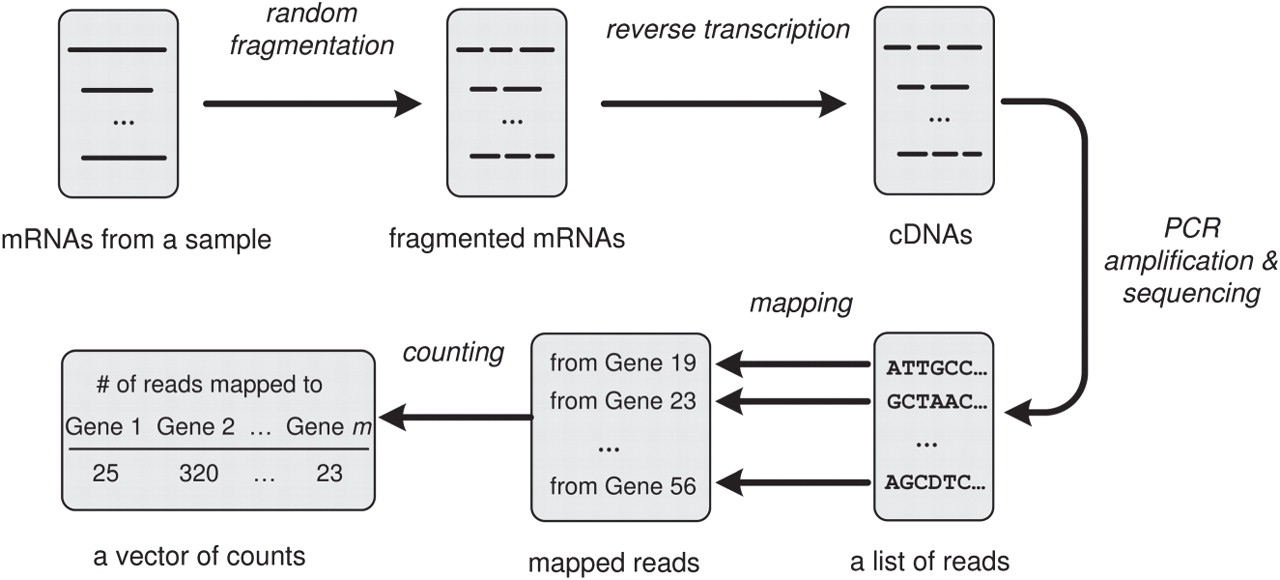
\includegraphics[width=0.9\textwidth]{pics/li-biostats12.jpg}
  \caption{Figure from Li et al., Normalization, testing, and false discovery rate estimation for RNA-sequencing data, Biostatistics, 2012, 13(3), by permission of Oxford University Press.}
  \label{fig:li-biostats}
\end{figure}


%%% Local Variables:
%%% TeX-master: "warwickthesis"
%%% End:
